% Lecture Template for ME3050 - Dynamic Modeling and Controls - Tennessee Technological University
% Spring 2024 - condensing and streamlining lectures by combining topics into a single PDF under the module name
% this will simplify file and link management as well as make lectures easier to use in class
% - added image/ to clean directory and reduce redundancy, specific to module for now  

% Module Name: - Frequency Response
% Topic 1 - Frequency Response of First Order Systems 
% Topic 2 - The Bode Diagram
% Topic 3 - Frequency Response of 2$^{nd}$ Order Systems
% Topic 4 - Resonance

\documentclass[fleqn]{beamer} % for presentation (has nav buttons at bottom)

%\usepackage{/home/tntech.edu/thill/courses/dmc/lectures/dmc_lectures}
%\usepackage{/home/thill/courses/dmc/lectures/dmc_lectures}
\usepackage{/mnt/c/Users/thill/Documents/courses/dmc/lectures/dmc_lectures}

\author{ME3050 - Dynamics Modeling and Controls}

\newcommand{\MNUM}{2\hspace{2mm}} % module number 
\newcommand{\moduletitle}{Frequency Response}

\newcommand{\sectionItitle}{Frequency Response of First Order Systems}
\newcommand{\sectionIItitle}{The Bode Diagram}
\newcommand{\sectionIIItitle}{Frequency Response of 2$^{nd}$ Order Systems}
\newcommand{\sectionIVtitle}{Resonance}

\newcommand{\sectionIsubsectionItitle}{Frequency Input Concept}
\newcommand{\sectionIsubsectionIItitle}{Complex Numbers Review}
\newcommand{\sectionIsubsectionIIItitle}{Frequency Response of First Order Systems}
\newcommand{\sectionIsubsectionIVtitle}{Graph of Frequency Response}

\newcommand{\sectionIIsubsectionItitle}{Review Frequency Response}
\newcommand{\sectionIIsubsectionIItitle}{Amplitude ratio in Decibels}
\newcommand{\sectionIIsubsectionIIItitle}{The Bode Diagram}
\newcommand{\sectionIIsubsectionIVtitle}{Frequency Response in MATLAB}

\newcommand{\sectionIIIsubsectionItitle}{Review Transfer Functions}
\newcommand{\sectionIIIsubsectionIItitle}{Frequency Response of Overdamped Systems}
\newcommand{\sectionIIIsubsectionIIItitle}{Frequency Response of Underdamped Systems}
\newcommand{\sectionIIIsubsectionIVtitle}{MATLAB Bode Plots}

\newcommand{\sectionIVsubsectionItitle}{Review 2$^{nd}$ Order Frequency Response}
\newcommand{\sectionIVsubsectionIItitle}{The Resonance Phenomenon}
\newcommand{\sectionIVsubsectionIIItitle}{The Resonance Frequency}
\newcommand{\sectionIVsubsectionIVtitle}{MATLAB Bode Plots}

\newcommand{\LT}{\mathcal{L}} % lagrangian

% custom box
\newsavebox{\mybox}

\title{Lecture Module - \moduletitle}

\date{Mechanical Engineering\vspc Tennessee Technological University}

\begin{document}

	\lstset{language=MATLAB,basicstyle=\ttfamily\small,showstringspaces=false}

	\frame{\titlepage \center\begin{framed}\Large \textbf{\moduletitle}\end{framed} \vspace{5mm}}

	% Module Outline
	\begin{frame} 
		\large \textbf{Lecture Module - \moduletitle} \vspace{3mm}\\

		\begin{itemize}
			\item Topic 1 - \hyperlink{sectionI}{\sectionItitle} \vspc % section I
			\item Topic 2 - \hyperlink{sectionII}{\sectionIItitle} \vspc % section II
			\item Topic 3 - \hyperlink{sectionIII}{\sectionIIItitle} \vspc % section III
			\item Topic 4 - \hyperlink{sectionIV}{\sectionIVtitle} \vspc % section IV
		\end{itemize}

	\end{frame}

	% section I
	\section{\sectionItitle}\label{sectionI}

		% section I Outline
		\begin{frame} 
			\large \textbf{Topic 1 - \sectionItitle} \vspace{3mm}\\

			\begin{itemize}
				\item \hyperlink{sectionIsubsectionI}{\sectionIsubsectionItitle} \vspc %  section I subsection I
				\item \hyperlink{sectionIsubsectionII}{\sectionIsubsectionIItitle} \vspc % section I subsection II
				\item \hyperlink{sectionIsubsectionIII}{\sectionIsubsectionIIItitle} \vspc % section I subsection III
				\item \hyperlink{sectionIsubsectionIV}{\sectionIsubsectionIVtitle} \vspc % section I subsection IV
			\end{itemize}
		\end{frame}
		
		% section I subsection I 
		\subsection{\sectionIsubsectionItitle}\label{sectionIsubsectionI}

			\begin{frame}
				\frametitle{\sectionIsubsectionItitle}
				\bigskip

					\small 
					The term {\bf frequency response} is used to describe a system's response to a periodic input. Frequency response analysis focuses on a system's response to {\it harmonic} input such as sines and cosines. The input (forcing) function is written below.\vspcc


					\begin{framed}
					\scalebox{1.25}{$f(t)=Asin\left(\omega t\right)$}\vspccc

					\renewcommand{\arraystretch}{1.5}
					\begin{tabular}{ccc}
					Amplitude of the Input, & \scalebox{1}{$A$} & \scalebox{1}{$ (N)$} \\
					Frequency of Input, &\scalebox{1}{$\omega$} &  \scalebox{1}{$(\frac{rad}{s})$}\\
					\end{tabular}
					\end{framed}

				\btVFill
			\end{frame}

			\begin{frame}
				\frametitle{\sectionIsubsectionItitle}
				\bigskip

				%\frametitle{Why Study Frequency Response?}
				\small
				 Why do we care about the way a system responds to harmonic excitation? Why is {\bf frequency analysis} important? \\
				\begin{itemize}
				\item
				\item
				\item
				\end{itemize}

				\vspace{3mm}What causes {\bf harmonic} (or sinusoidal) excitation in the real world? \\

				\begin{itemize}
				\item
				\item
				\item
				\end{itemize}
 
				\btVFill
			\end{frame}

			\begin{frame}
				\frametitle{\sectionIsubsectionItitle}
				\bigskip

				%\frametitle{Frequency Response and the Transfer Function}

				A linear, time-invariant (LTI) system has a {\bf transfer function} $T(s)$ that describes the {\bf input-output} relationship of the system. Under sinusoidal excitation (input) with frequency $\omega$ if the system is stable the transient affects in the response (output) will eventually disappear leaving the {\bf steady state sinusoidal response} of the same frequency as the input but with a phase shift w.r.t. the input.


				\btVFill
			\end{frame}

		



		% section I subsection II
		\subsection{\sectionIsubsectionIItitle}\label{sectionIsubsectionII}

			\begin{frame}
				\frametitle{\sectionIsubsectionIItitle}
				\bigskip

				%\frametitle{The Complex Plane}

				In an underdamped system the roots of the characteristic polynomial are complex. Before we proceed we need to review some rules of arithmetic and complex numbers. \vspc

				\begin{multicols}{2}
				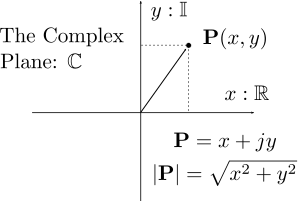
\includegraphics[scale=0.175]{images/lecture1_fig1.png}

				\small
				\hspccc Cartesian Representation:\vspc\hspccc\scalebox{.8}{$\mathbf{P}=x+jy$}\vspc
				\hspccc Polar Representation:\vspc\hspccc\scalebox{.8}{$\mathbf{P}=|\mathbf{P}|\angle\theta$}\vspc
				\hspccc Exponential Representation:\vspc\hspccc\scalebox{.8}{$\mathbf{P}=|\mathbf{P}|e^{j\theta}=|\mathbf{P}|\left(cos\theta+jsin\theta\right)$}\vspc
				\end{multicols}

				\btVFill
			\end{frame}

				%\btVFill
			\begin{frame}
				\frametitle{\sectionIsubsectionIItitle}
				\bigskip

				\frametitle{Complex Number Algebra}
 
				 Consider two points $\mathbf{P_1}$ and $\mathbf{P_2}$ on the complex plane. \vspc
				 
				 \scalebox{1}{$\mathbf{P_1}=x_1+jy_1$\hspc and \hspc$\mathbf{P_2}=x_2+jy_2$} \vspccc
				\renewcommand{\arraystretch}{1.75}
				 \begin{tabular}{cc}
				 Addition:& \scalebox{1}{$\mathbf{P_1}+\mathbf{P_2}=(x_1+x_2)+j(y_1+y_2)$}\\
				 Multiplication:& \scalebox{1}{$\mathbf{P_1P_2}=|\mathbf{P_1P_2}|\angle\left(\theta_1+\theta_2\right)$}\\
				 Division:&\scalebox{1}{$\frac{\mathbf{P_1}}{\mathbf{P_2}}=(x_1+x_2)+j(y_1+y_2)$}\\
				\end{tabular}
				
				\btVFill
			\end{frame}

		% section I subsection III
		\subsection{\sectionIsubsectionIIItitle}\label{sectionIsubsectionIII}
			\begin{frame} 
				\frametitle{\sectionIsubsectionIIItitle}
				\bigskip

				\frametitle{First Order Mass Damper}

				\includegraphics[scale=.15]{images/porsche.png}

				Consider our $1^{\underline{st}}$ order mass damper system. \vspc

				\scalebox{1}{$m\dot{v}+cv=f(t)$} \hspcc with a {\bf time constant} \scalebox{1}{$\tau=\frac{m}{c}$} \vspcc

				The system is commonly re-written as shown below. \vspc

				\scalebox{1}{$m\dot{v}+cv=f(t)\hspc\rightarrow\hspc\tau\dot{y}+y=f(t)$} \vspc

				\btVFill
			\end{frame}	

			\begin{frame} 
				\frametitle{\sectionIsubsectionIIItitle}
				\bigskip

				\frametitle{First Order Transfer Function}

				\small

				\scalebox{1}{$\tau\dot{y}+y=f(t)$} \vspcc

				Take the Laplace transform of the ODE. \vspcc

				\scalebox{1}{$\LT\{\tau\dot{y}+y\}=\LT\{f(t)\}$} \vspcc

				\scalebox{1}{$\tau\left(sY(s)+y_0)\right)+Y(s)=F(s)$}\hspccc The initial conditions are zero. \vspcc

				\begin{framed}
				\scalebox{1}{$T(s)=\frac{Y(s)}{F(s)}=\frac{1}{\tau s+1}$}\hspccc First Order Transfer Function
				\end{framed}

				This considers a {\it generalized} input function $f(t)$ and zero ICs.
				\btVFill
			\end{frame}	

		% section I subsection IV
		\subsection{\sectionIsubsectionIVtitle}\label{sectionIsubsectionIV}

			\begin{frame}
				\frametitle{\sectionIsubsectionIVtitle}
				\bigskip

				\frametitle{Sinusoidal Input Function}

				\small

				Our model is now excited by a sinusoidal input function. \vspc

				\scalebox{1}{$\tau\dot{y}+y=f(t)=Asin\left(\omega t\right)$} \vspc

				Take the Laplace transform. Then, solve for $Y(s)$ and expand.\vspc

				\scalebox{1}{$\tau sY(s)+Y(s)=\frac{A\omega}{s^2+\omega^2}$}  \vspc

				\scalebox{1}{$Y(s)=\frac{A\omega}{\left(s^2+\omega^2\right)\left(\tau s+1\right)}=\frac{C_1}{\tau s+1}+\frac{C_2s}{\left(s^2+\omega^2\right)}+\frac{C_3\omega}{\left(s^2+\omega^2\right)}$} \vspc

				Now solve for the coefficients.\vspc

				\scalebox{1}{$C_1=\frac{A\omega\tau^2}{1+\omega^2\tau^2}\hspccc,\hspc C_2=\frac{-A\omega\tau}{1+\omega^2\tau^2}\hspccc,\hspc C_3=\frac{A}{1+\omega^2\tau^2}$} \vspc

				Substituting and take the inverse Laplace transform. \vspc
				\scalebox{1}{$y(t)=\frac{A\omega\tau}{1+\omega^2\tau^2}\big( e^{\frac{-t}{\tau}}-cos\omega t+\frac{1}{\omega\tau}sin\omega t\big) $}
		
				\btVFill
			\end{frame}	

			\begin{frame}
				\frametitle{\sectionIsubsectionIVtitle}
				\bigskip

				\frametitle{Steady State Time Response}

				\small
				\scalebox{1}{$y(t)=\frac{A\omega\tau}{1+\omega^2\tau^2}\big( e^{\frac{-t}{\tau}}-cos\omega t+\frac{1}{\omega\tau}sin\omega t\big) $} \vspcc
				After some amount of time passes, the transient term will disappear leaving just the sinusoidal terms. \vspcc

				\scalebox{1}{$y(t)=\frac{A}{1+\omega^2\tau^2}\big(sin\omega t - \omega\tau cos\omega t\big) $} \vspccc
				This is re-written as a single sine term with a phase shift. \vspc

				\begin{framed}
				Steady State Frequency Response of First Order System\vspc
				\scalebox{1}{$y(t)=\frac{A}{\sqrt{1+\omega^2\tau^2}}sin\left(\omega t+\phi\right) \hspccc,\hspc \phi=-tan^{-1}\omega\tau$}
				\end{framed}

				\btVFill
			\end{frame}	

			\begin{frame}
				\frametitle{\sectionIsubsectionIVtitle}
				\bigskip
				\frametitle{Amplitude Ratio}

				\small

				\scalebox{1}{$y(t)=\frac{A}{\sqrt{1+\omega^2\tau^2}}sin\left(\omega t+\phi\right) \hspccc,\hspc \phi=-tan^{-1}\omega\tau$} \vspc

				Notice that the system responds at the same frequency as the input but with a different amplitude and a phase shift. The ratio of the response amplitude to the input amplitude is called the {\bf amplitude ratio, M}. \vspc

				\scalebox{1}{$M=\frac{\frac{A}{\sqrt{1+\omega^2\tau^2}}}{A}=\frac{1}{\sqrt{1+\omega^2\tau^2}}$} \vspc

				Fortunately we can find the {\bf amplitude ratio} and {\bf phase shift} directly from the transfer function. Recall the transfer function we derived. \vspc

				\scalebox{1}{$T(s)=\frac{1}{\tau s+1}$}\hspccc let \scalebox{1}{$s=j\omega\hspccc\implies\hspccc T(j\omega)=\frac{1}{\tau j\omega+1}$} \vspc

				\scalebox{1}{$|T(j\omega)|=\frac{|1|}{|\tau j\omega+1|}=\frac{1}{\sqrt{\left(\tau\omega\right)^2+1^2}}=\frac{1}{\sqrt{1+\tau^2\omega^2}}$} \hspccc \hspccc Look familiar? \vspc 

				\btVFill
			\end{frame}

			\begin{frame}
				\frametitle{\sectionIsubsectionIVtitle}
				\bigskip
				\frametitle{Phase Angle}		
				\small

				\scalebox{1}{$|T(j\omega)|=\frac{1}{\sqrt{1+\tau^2\omega^2}}=M(\omega)$}\vspc

				\scalebox{1}{$\angle T\left(j\omega\right)=\angle 1-\angle\left(1+j\omega\tau\right)=tan^{-1}\left(\frac{0}{1}\right)-tan^{-1}\left(\frac{\omega\tau}{1}\right)=$}\vspc
				\scalebox{1}{$-tan^{-1}\left(\omega\tau\right)=\phi(\omega)$}\vspcc

				Substitute $s=j\omega$ into the transfer function and solve for the magnitude and phase angle of this complex number which represent the magnitude ratio and phase shift. \vspc

				Therefore the steady state response is written as follows.  \vspc

				\scalebox{1}{$y_{ss}\left(t\right)=A|T\left(j\omega\right)|sin\left(\omega t+\angle T\left(j\omega\right)\right)=MAsin\left(\omega t+\phi\right)$}\vspcc

				Wasn't that fun? Can you believe we used to do that on the board?!?! \vspc

				\btVFill
			\end{frame}
	
	% Section II
	\section{\sectionIItitle}\label{sectionII}

		% section II Outline
		\begin{frame}
			\large \textbf{Topic 2 - \sectionIItitle} \vspace{3mm}\\

			\begin{itemize}
				\item \hyperlink{sectionIIsubsectionI}{\sectionIIsubsectionItitle} \vspc %  section II subsection I
				\item \hyperlink{sectionIIsubsectionII}{\sectionIIsubsectionIItitle} \vspc % section II subsection II
				\item \hyperlink{sectionIIsubsectionIII}{\sectionIIsubsectionIIItitle} \vspc % section II subsection III
				%\item \hyperlink{sectionIIsubsectionIV}{\sectionIIsubsectionIVtitle} \vspc % section II subsection IV
			\end{itemize}

		\end{frame}

		% section II subsection I
		\subsection{\sectionIIsubsectionItitle}\label{sectionIIsubsectionI}

			\begin{frame}[label=sectionIIsubsectionI]
				\frametitle{\sectionIIsubsectionItitle}
				\bigskip

				
				\btVFill
			\end{frame}


		% section II subsection II
		\subsection{\sectionIIsubsectionIItitle}\label{sectionIIsubsectionII}

			\begin{frame}

				\frametitle{\sectionIIsubsectionIItitle}
				\bigskip

				\btVFill 
			\end{frame}

			\begin{frame}

				\frametitle{\sectionIIsubsectionIItitle}
				\bigskip



				\btVFill 
			\end{frame}




		% section II subsection III
		\subsection{\sectionIIsubsectionIIItitle}\label{sectionIIsubsectionIII}

			\begin{frame}
				\frametitle{\sectionIIsubsectionIIItitle}
				\bigskip

			
				\btVFill 
			\end{frame}	


			\begin{frame}
				\frametitle{\sectionIIsubsectionIItitle}
				\bigskip

				
				
				\btVFill 
			\end{frame}	


			\begin{frame}
				\frametitle{\sectionIIsubsectionIIItitle}
				\bigskip

				
				\btVFill 
			\end{frame}

			
		% section II subsection IV
		\subsection{\sectionIIsubsectionIVtitle}\label{sectionIIsubsectionIV}

			\begin{frame}
				\frametitle{\sectionIIsubsectionIVtitle}
				\bigskip
				

				\btVFill 
			\end{frame}	

			\begin{frame}
				\frametitle{\sectionIIsubsectionIVtitle}
				\bigskip
				

				\btVFill 
			\end{frame}	

			\begin{frame}
				\frametitle{\sectionIIsubsectionIVtitle}
				\bigskip
			

				\btVFill 
			\end{frame}	


		
	% Section III
	\section{\sectionIIItitle}\label{sectionIII}

		% section III Outline
		\begin{frame}
			\large \textbf{Topic 3 - \sectionIIItitle} \vspace{3mm}\\

			\begin{itemize}
				\item \hyperlink{sectionIIIsubsectionI}{\sectionIIIsubsectionItitle} \vspc %  section III subsection I
				\item \hyperlink{sectionIIIsubsectionII}{\sectionIIIsubsectionIItitle} \vspc % section III subsection II
				\item \hyperlink{sectionIIIsubsectionIII}{\sectionIIIsubsectionIIItitle} \vspc % section III subsection III
				\item \hyperlink{sectionIIIsubsectionIV}{\sectionIIIsubsectionIVtitle} \vspc % section III subsection IV
				%\item \hyperlink{sectionIIIsubsectionV}{\sectionIIIsubsectionVtitle} \vspc % section III subsection V
			\end{itemize}

		\end{frame}

		% section III subsection I
		\subsection{\sectionIIIsubsectionItitle}\label{sectionIIIsubsectionI}

			\begin{frame}
				\frametitle{\sectionIIIsubsectionItitle}
				\bigskip


				\btVFill
			\end{frame}

			\begin{frame}
				\frametitle{\sectionIIIsubsectionItitle}
				\bigskip
				

				\btVFill
			\end{frame}

		% section III subsection II
		\subsection{\sectionIIIsubsectionIItitle}\label{sectionIIIsubsectionII}	

			\begin{frame}
				\frametitle{\sectionIIIsubsectionIItitle}
				\bigskip

	
				\btVFill
			\end{frame}

		% section III subsection III
		\subsection{\sectionIIIsubsectionIIItitle}\label{sectionIIIsubsectionIII}

			\begin{frame}
				\frametitle{\sectionIIIsubsectionIIItitle}
				\bigskip

		
			
				\btVFill
			\end{frame}

			\begin{frame}
				\frametitle{\sectionIIIsubsectionIIItitle}
				\bigskip

			
				\btVFill
			\end{frame}

		% section III subsection IV
		\subsection{\sectionIIIsubsectionIVtitle}\label{sectionIIIsubsectionIV}	

			\begin{frame}
				\frametitle{\sectionIIIsubsectionIVtitle}
				\bigskip

				

				\btVFill 
			\end{frame}

			\begin{frame}
				\frametitle{\sectionIIIsubsectionIVtitle}
				\bigskip

			

		 		\btVFill 
			\end{frame}
			
			\begin{frame}
				\frametitle{\sectionIIIsubsectionIVtitle}
				\bigskip
				
				
					
				\btVFill 
			\end{frame}

			\begin{frame}
				\frametitle{\sectionIIIsubsectionIVtitle}
				\bigskip
			
				
				\btVFill 
			\end{frame}
    

	% Section IV
	\section{\sectionIVtitle}\label{sectionIV}

		% section IV Outline
		\begin{frame}
			\large \textbf{Topic 3 - \sectionIVtitle} \vspace{3mm}\\

			\begin{itemize}
				\item \hyperlink{sectionIVsubsectionI}{\sectionIVsubsectionItitle} \vspc %  section III subsection I
				\item \hyperlink{sectionIVsubsectionII}{\sectionIVsubsectionIItitle} \vspc % section III subsection II
				\item \hyperlink{sectionIVsubsectionIII}{\sectionIVsubsectionIIItitle} \vspc % section III subsection III
				\item \hyperlink{sectionIVsubsectionIV}{\sectionIVsubsectionIVtitle} \vspc % section III subsection IV

			\end{itemize}

		\end{frame}

		% section IV subsection I
		\subsection{\sectionIVsubsectionItitle}\label{sectionIVsubsectionI}

			\begin{frame}
				\frametitle{\sectionIVsubsectionItitle}
				\bigskip


				\btVFill
			\end{frame}

			\begin{frame}
				\frametitle{\sectionIVsubsectionItitle}
				\bigskip
				

				\btVFill
			\end{frame}

		% section IV subsection II
		\subsection{\sectionIVsubsectionIItitle}\label{sectionIVsubsectionII}	

			\begin{frame}
				\frametitle{\sectionIVsubsectionIItitle}
				\bigskip

	
				\btVFill
			\end{frame}

		% section IV subsection III
		\subsection{\sectionIVsubsectionIVtitle}\label{sectionIVsubsectionIV}

			\begin{frame}
				\frametitle{\sectionIVsubsectionIVtitle}
				\bigskip

		
			
				\btVFill
			\end{frame}

			\begin{frame}
				\frametitle{\sectionIVsubsectionIVtitle}
				\bigskip

			
				\btVFill
			\end{frame}

		% section IV subsection III
		\subsection{\sectionIVsubsectionIIItitle}\label{sectionIIIsubsectionIV}	

			\begin{frame}
				\frametitle{\sectionIVsubsectionIIItitle}
				\bigskip

				

				\btVFill 
			\end{frame}

			\begin{frame}
				\frametitle{\sectionIVsubsectionIIItitle}
				\bigskip

			

		 		\btVFill 
			\end{frame}
			
			\begin{frame}
				\frametitle{\sectionIVsubsectionIIItitle}
				\bigskip
				
				
					
				\btVFill 
			\end{frame}

			\begin{frame}
				\frametitle{\sectionIVsubsectionIIItitle}
				\bigskip
			
				
				\btVFill 
			\end{frame}



\end{document}





